\chapter{Evaluation\label{chap:evaluation}}


%Explain simulation and communication
%Evaluate different models task based
%How where the realisations/ideas tested?
%What were the results of those tests?

The implementations of the developed concepts were evaluated with regard to the three requirements stated in the introduction: 
\begin{itemize}
\item Update models incrementally during the interaction
\item Prediction of future object states
\item Incrementally reach a given target configuration
\end{itemize}

In order to evaluate these requirements, the implementations are tested in two different tasks using a physics simulation. The first task, the \textit{Push Task Simulation} tests the forward models of the different implementations. The actual task as well as the results achieved in that task are explained in section \ref{sec:pushTaskSim}.
The second task, \textit{Move to Target}, tests the implementations' ability to move an object towards a given configuration. This task and its results are explained in section \ref{sec:moveToTarget}.
Both tasks are evaluated using different settings for the implementations.

The used simulation software as well as the simulated environment are explained in section \ref{sec:environment}.


\section{Simulation and environment \label{sec:environment}}

The model is supposed to learn object manipulation through interaction.
The developed prototype implementations are tested in a simplified simulation. For this work gazebo \cite{gazebo} version 2.2.3 was used with the physics engine Open Dynamics Engine (ODE) \cite{ode}.
Gazebo simulates physics one step at a time at fixed time intervals. It is possible to configure the maximum step size for each update step as well as the number of steps to be performed in one second in real time. 
The simulation time depends on these to values. For this thesis, the standard step size of 0.001 simulation seconds is used. The \enquote{real time update rate}, which determines how many steps are performed in one second in real time, is used to control the speed at which the simulation is performed. 
This thesis uses an update rate of 500 when the models are to be updated at 100Hz according to simulation time. By setting the update rate to that half of real time, the models have 0.02 seconds in real time in order to finish their updates and queries. %TODO consider redoing or moving elsewhere
The simulation sends information about the objects every x steps, where x depends on the chosen update rate and step size. When using 100Hz, the simulation publishes the objects' information every 10 steps.

A very simple two dimensional environment is used, only containing a spherical actuator and a rectangular cube object that can be seen in figure \ref{fig:gazeboWorld}.
The dimensions of all objects as well as their friction coefficients used by the physics simulation are listed in table \ref{tab:environmentObjects}.
The fairly high friction coefficient for the block was chosen in order to better suit the assumption of the object state model. By increasing the friction the block will
slide less. 

\begin{table}
	\centering
	\begin{tabular*}{\textwidth}{@{\extracolsep{\fill} } c c c c}
			\hline \textbf{Object} & \textbf{Dimension} & \multicolumn{2}{c}{\textbf{Friction coefficients}} \\ 
			\multicolumn{2}{c}{} & $\mu_1$ & $\mu_2$ \\
			\hline \hline 
			 Actuator & $0.025m$ & 0.01 & 0.01 \\
			 Blue rectangular cube & $0.5m \times 0.1m \times 0.1m$ & 0.9 & 0.9 \\  
			\hline 
	\end{tabular*} 
	\caption{Table summarizing the dimensions and friction coefficients for the objects in the environment. If only one dimension is given, it represents the radius. Three dimensions correspond to the width, depth and height of an object.}
	\label{tab:environmentObjects}
\end{table}

\begin{figure} 
	\centering
	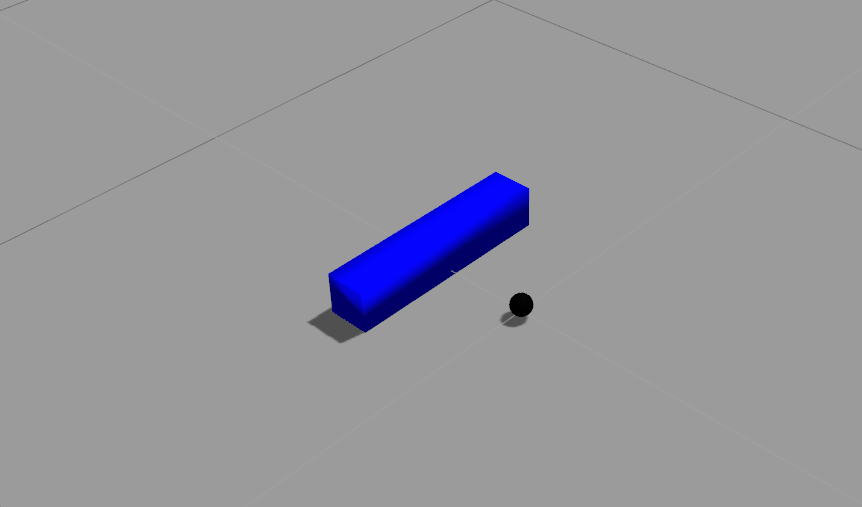
\includegraphics[width=10cm]{gazeboWorld.png} 
	\caption{Overview of the used environment. The black sphere represents the actuator, the models can control using action primitives. The blue square represents the object that the actuator interacts with.}
	\label{fig:gazeboWorld}
\end{figure}


\subsection{Communication}
Gazebo uses a client-server architecture. The actual simulation is being performed by the server.
This server publishes Google Protobuf \cite{protobuf} messages via TCP/IP. Interested clients, for example a graphical user interface, can register themselves as listener to messages of desired types. 
It is also possible to send messages to the server in order to influence the simulation. 

The server can furthermore be extended by writing custom plug-ins that handle self defined messages or perform some sort of additional computation at each update step of the simulation. 

In order for the Python prototypes to communicate with the simulation, an interface on both sides was created.

On the side of the simulation, a custom server plug-in was written, that publishes the information described in table \ref{tab:availInformation} in the realization chapter. 
The server publishes the 
The information for all objects is packed into a custom Protobuf message, which is explained in details in Appendix \ref{sec:protobufMessages}. Basically, this message simply contains a list of object descriptions where each object description contains the information explained in table \ref{tab:availInformation}.
Furthermore, the plug-in receives custom control messages. These messages allow the Python interface to influence the simulation.
While the exact messages are explained in the Appendix \ref{sec:protobufMessages}, table \ref{tab:commands} gives an overview about the possible commands, that can be send to the simulation.

On the Python side, an interface was written with the help of the module pygazebo \cite{pygazebo}, which provides Python bindings for the message passing system used by gazebo. This interface handles the messages that are received from and send to the simulation. 
The simulation sends information about the objects at a fixed rate. At each update step, the interface performs four to five actions:
\begin{enumerate}
\item Construct a suitable worldstate from the provided information
\item Get a prediction about the next worldstate from the model using the current worldstate
\item Update the model with the current worldstate
\item Get an action primitive from the model given a target configuration
\item Send the current action primitive to the simulation
\end{enumerate}

The 4th step is only performed in the tasks evaluating the inverse model. In the \textit{Push Task Simulation} a fixed action primitive is predetermined.

Furthermore, the Python interface provides the testing framework of setting up the models and managing training and testing runs as explained in detail below.

\begin{table}
	\centering
	\begin{tabular}{|c|c|}
		\hline \textbf{Command} & \textbf{Meaning} \\ 
		\hline Move Command & Sets the velocity for the actuator \\ 
		\hline Pause & Pauses the simulation \\
		\hline Continue & Continues the simulation \\
		\hline Reset & Resets the world to starting configuration \\
		\hline Set Pose & Places a specified object at a certain position \\
		\hline
	\end{tabular} 
	\caption{Overview of all implemented commands to influence the simulation.}
	\label{tab:commands}
\end{table}

\subsection{Sources of noise}

Although the object's attributes can be read accurately from the simulation, some random noise is still present in the data: \\
1) The physics simulation and the sensors that record the object's attribute are run in different threads within
in the simulation. These threads cannot always be perfectly synchronized which can result in minor differences in consecutive 
timesteps. \\
2) The physics simulation itself might encounter numerical instabilities, especially when computing resting forces. These instabilities
might lead to small oscillations within an object's features, such as position. In order to filter out such small noise, all
information from the simulation is rounded to 3 decimal places while constructing the worldstate. \\
3) The strongest variation comes from the fact that the implementation communicates with the simulation via asynchronous messages. 
All runs start in a configuration where all objects are resting. In the very first update step, the Python interface sends the first
action primitive to the simulation, which results in the actuator moving. The exact time when the simulation retrieves and executes
the action is however not deterministic. Depending on the system's load the simulation might have already performed 5 update steps before
it receives and executes the action. In this case, the action affects only half of the update steps. In another situation, the action might
be executed earlier. From the model's point of view, the same action was performed from the same initial situation, but the results can
differ greatly. 

Since this thesis considers a rather simple scenario and these three sources of noise are already present due to the used technologies,
no additional artificial noise was introduced to the system.

\section{Push Task Simulation \label{sec:pushTaskSim}}

%The first set of evaluations targets the prediction performance of the models. 

\subsection{Scenario description}

In this task, the actuator uses a constant action in order to first move towards the block and then push it.
The actuator starts at different starting positions on a line parallel to the block so that the distance along
the action axis always starts at 25cm between the two centers. The block is orientated so that it's main axis
is perpendicular to the action axis.

The model is first trained using the open loop. This means that the model receives all information about the
world at each timestep before making the prediction for the next timestep. This training is done for a set amount
of \enquote{runs}. A run starts when the actuator performs the first action from the starting position and ends after a fixed 
number of iterations or if the actuator travels a predefined distance.
An example starting and end configuration can be seen in figure \ref{fig:pushTaskSim}. 

All starting positions except the first three are chosen randomly, but using the
same seed for all models and configurations. %TODO does not work, not even with the same model just with state3 vs state4... investigate!
The first three are chosen so that the actuator touches the object on the outer left, the outer right side
and directly at the center. This has been done to ensure that the models have seen all general interactions for when they are evaluated with only 3
runs. The random start positions are chosen in such a range, that the actuator can also pass the object without touching it, by sampling starting positions
between -0.35 and 0.35. Another seed is set after the training is done, so that all models are tested on the same starting positions, regardless of
the number of training examples.

The number of iterations used here is 150 when using
the model at 100Hz. During these iterations the actuator moves approximately 75cm. The maximal distance is set to 1m when using the
model with 10Hz. The actual action is the same for both frequencies and is that to 0.5m/s upwards towards the block from the starting
position. 

\begin{figure}
	%TODO make figure !
	
	\caption{TODO Push Task Simulation. The left side shows one exemplary start configuration, while on the right the corresponding end configuration can be seen.
		The darker objects (dark blue and black) represent the actual block and actuator, while the transparent objects symbolize the predicted objects.}
	\label{fig:pushTaskSim}
\end{figure}


\subsection{Evaluation criteria}

This task tries to evaluate the precision of the different models. In order to measure this precision, the predicted actuator position
is compared with the actual actuator position. Since at least the block can also rotate around the third axis, the orientation needs to be
considered as well when measuring the prediction performance. Since it is hard to find a metric that adequately combines point differences with
angular differences, the orientation is indirectly measured. In addition to the center position of each object, two key points are defined that
are located at the edges of the block as can be seen in figure \ref{fig:refPoints}. This way the euclidean distance can be used to measure the
prediction accuracy of both the object's position as well as their orientation. The three distances are then averaged to compute the final difference
score s:


where $p^{pred}_i, pred^{actual}_i$ represents the i's predicted and actual reference point, including the center, respectively.

These scores are computed at each timestep and accumulated. Furthermore, the final difference, at the last timestep of each run is recorded separately.
The results show the averaged results for the final difference, the accumulated differences and the mean difference over 20 test runs. The mean difference
is computed by dividing the accumulated difference by the number of predictions, the model made in each run, which is equal to the number of iterations-1. For the
first iteration, there has not been a prediction that can be compared yet.

\subsection{Results}

%TODO Also test only interaction prediction performance, by removing all the instances where only the gripper moved!



\section{Move to target \label{sec:moveToTarget}}

\subsection{Scenario description}

\subsection{Evaluation criteria}

\subsection{Results}